\chapter{Architecture}\label{Chap:Architecture}
\begin{figure}[!htb]
   \centering
   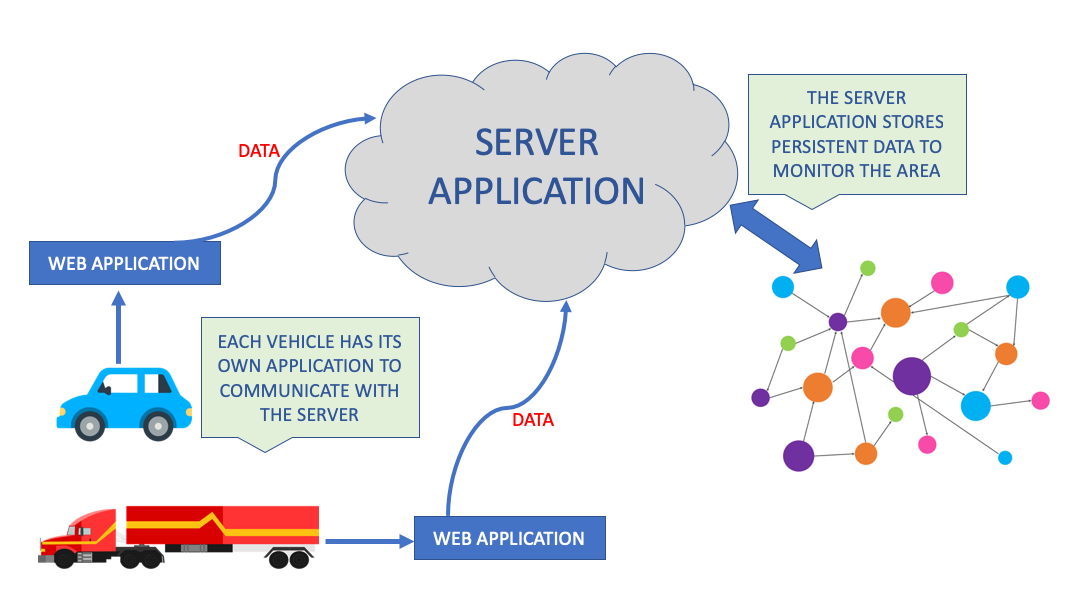
\includegraphics[width=\textwidth]{architecture.png}
   \caption{Architecture of the system.}\label{Fig:ArchNoImpl}
\end{figure}
As the figure \ref{Fig:ArchNoImpl} shows, the system consists of three principal components:
\begin{itemize}
  \item \underline{server}: this component is responsible for the validation of data, supervision of the system and interaction with the database
    to store persistent data;
  \item \underline{client}: this component consist of an application, located on the vehicle that communicates with the server and provide it with
    information about the vehicle (e.g. position, entry and exit time);
  \item \underline{database}: here the server application stores data about the current state of the area, i.e. actual capacity of places, position of vehicles,
  average times spent in each place.
\end{itemize}
